
\section{Implementation and processing details in Hercules}

Equivalent linear method is a set of iterative linear simulations which the material properties are being updated based on the strain level of previous simulation. The methodology and implementation of the method in 1D is well presented in different resources (e.g., see \citet{Kramer1996geotechnical}). In this section we explain the procedure that we have implemented in the model. In we defined specific elements to get updated due to equivalent linear process. These elements are mostly have low shear wave velocity and is defined by the user in the input parameters. Effective strain of each element is computed and stored for the element. At the end of each iteration, based on the user-defined shear modulus degradation curve, we compute the updated shear modulus for that element. Accordingly, S and P wave velocity of the element are updated. Internal friction or intrinsic attenuation in Hercules is addressed through BKT2 damping model. Hercules accept the damping as a Q-factor and convert it into damping for each parameters.  Updating process for damping is according the following steps:

\begin{itemize}
 \item step1: Storing the original Q value for all elements.
 \item step2: Converting the Q value into damping and add the new damping that is related to effective strain of the element and damping curve.
\begin{equation}
\xi_{an}=\frac{1}{2*Q_s}, 
\xi_{t}=\xi_{an} + \xi_{eq},
\end{equation}
\item step3: Converting the damping into Q factor and updating the Q value of the element. 
\begin{equation}
Q_{s,updated} = \frac{1}{2*\xi_{t}}
\end{equation}
\end{itemize}

In this study we only update the Qs value. Qp value is being updated accordingly.  


\subsection{Number of equivalent linear iteration}

Equivalent linear method is based on iteration and updating material. In theory we need to stop the simulation when the variation between effective strain in each element is less than a user defined value. Another option is to control the peak value of several stations. Therefore, we conduct a test to see how many iteration is necessary to reach to a stable results. The test is done in spherical basin 3, with point source 3. I present the results for station at the surface and at the depth of 64 m. According to these figures, the results become stable after five iterations. Fig.~\ref{fig:iteration_surface} and Fig.~\ref{fig:iteration_deep_64}  show the results for a station at the surface and depth of 64 m, respectively.


\begin{figure}[H]
    \centering
    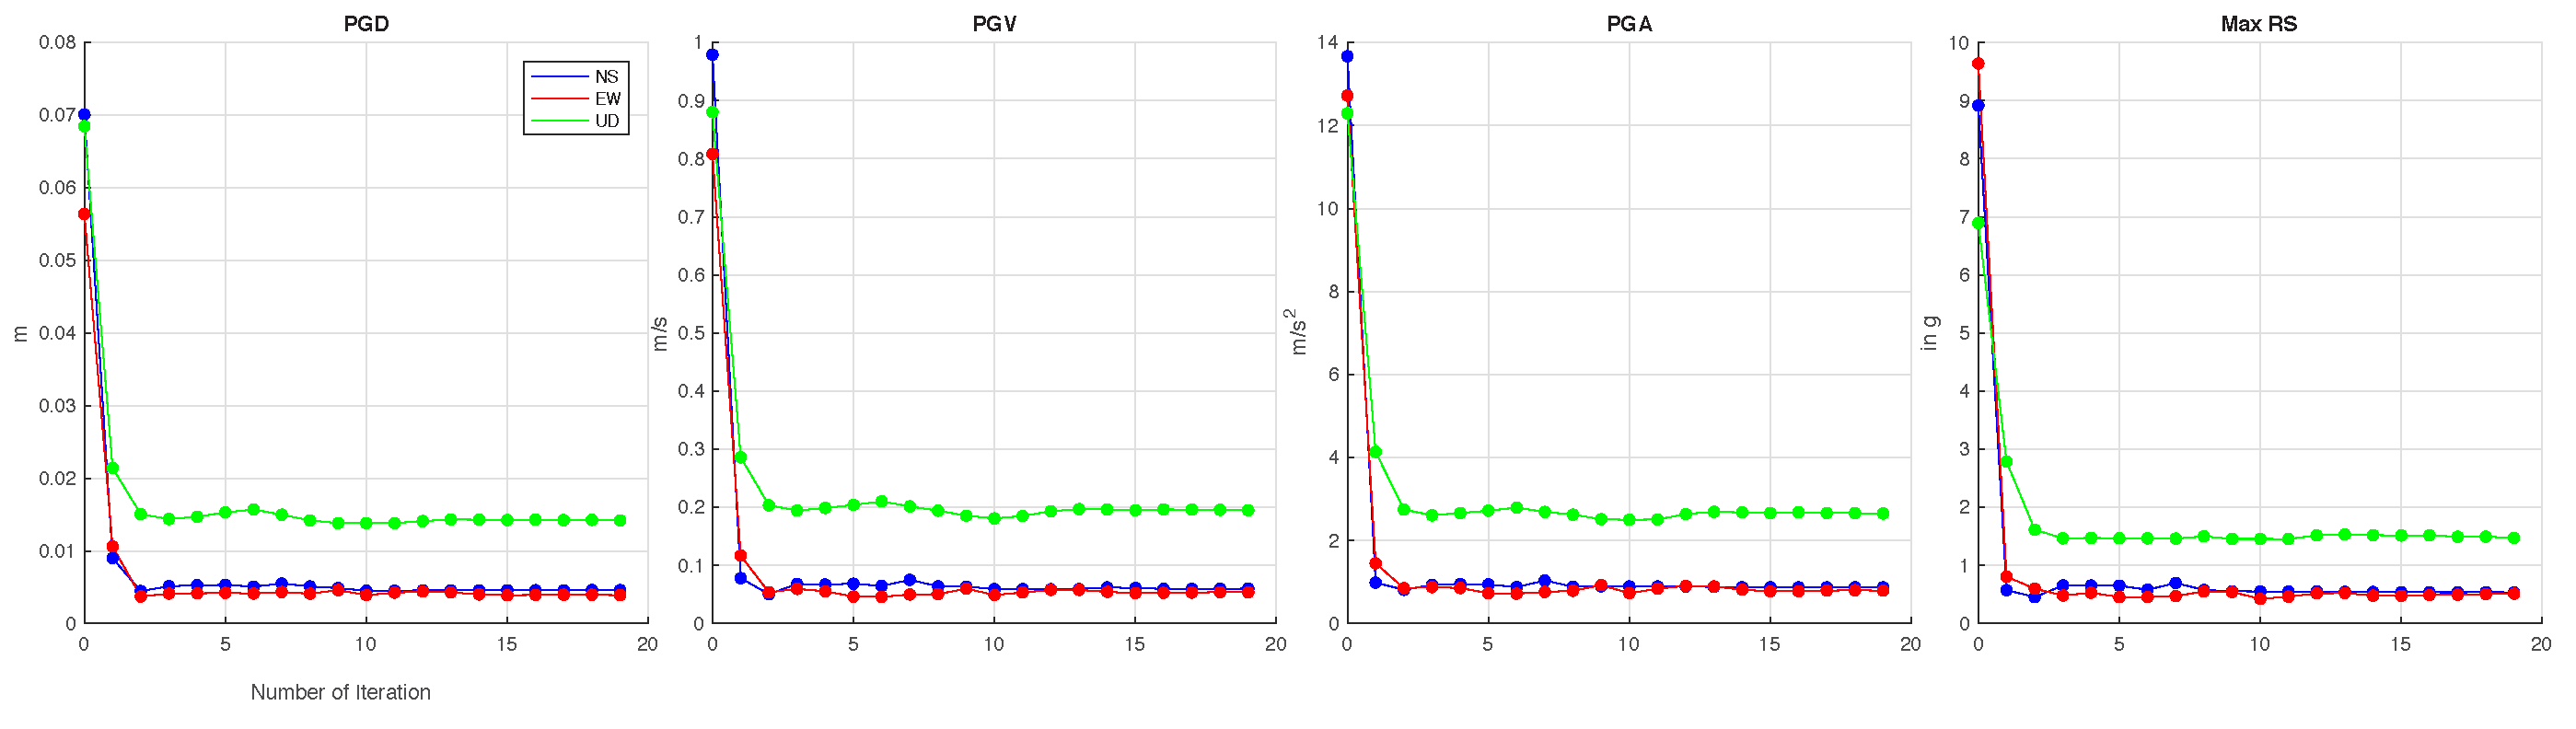
\includegraphics[width=\textwidth]{figures/pdf/iteration_surface.pdf}
    \caption{Analysis of stability of results in different iteration. Stations at the surface of the basin.}
    \label{fig:iteration_surface}
\end{figure}


\begin{figure}[H]
    \centering
    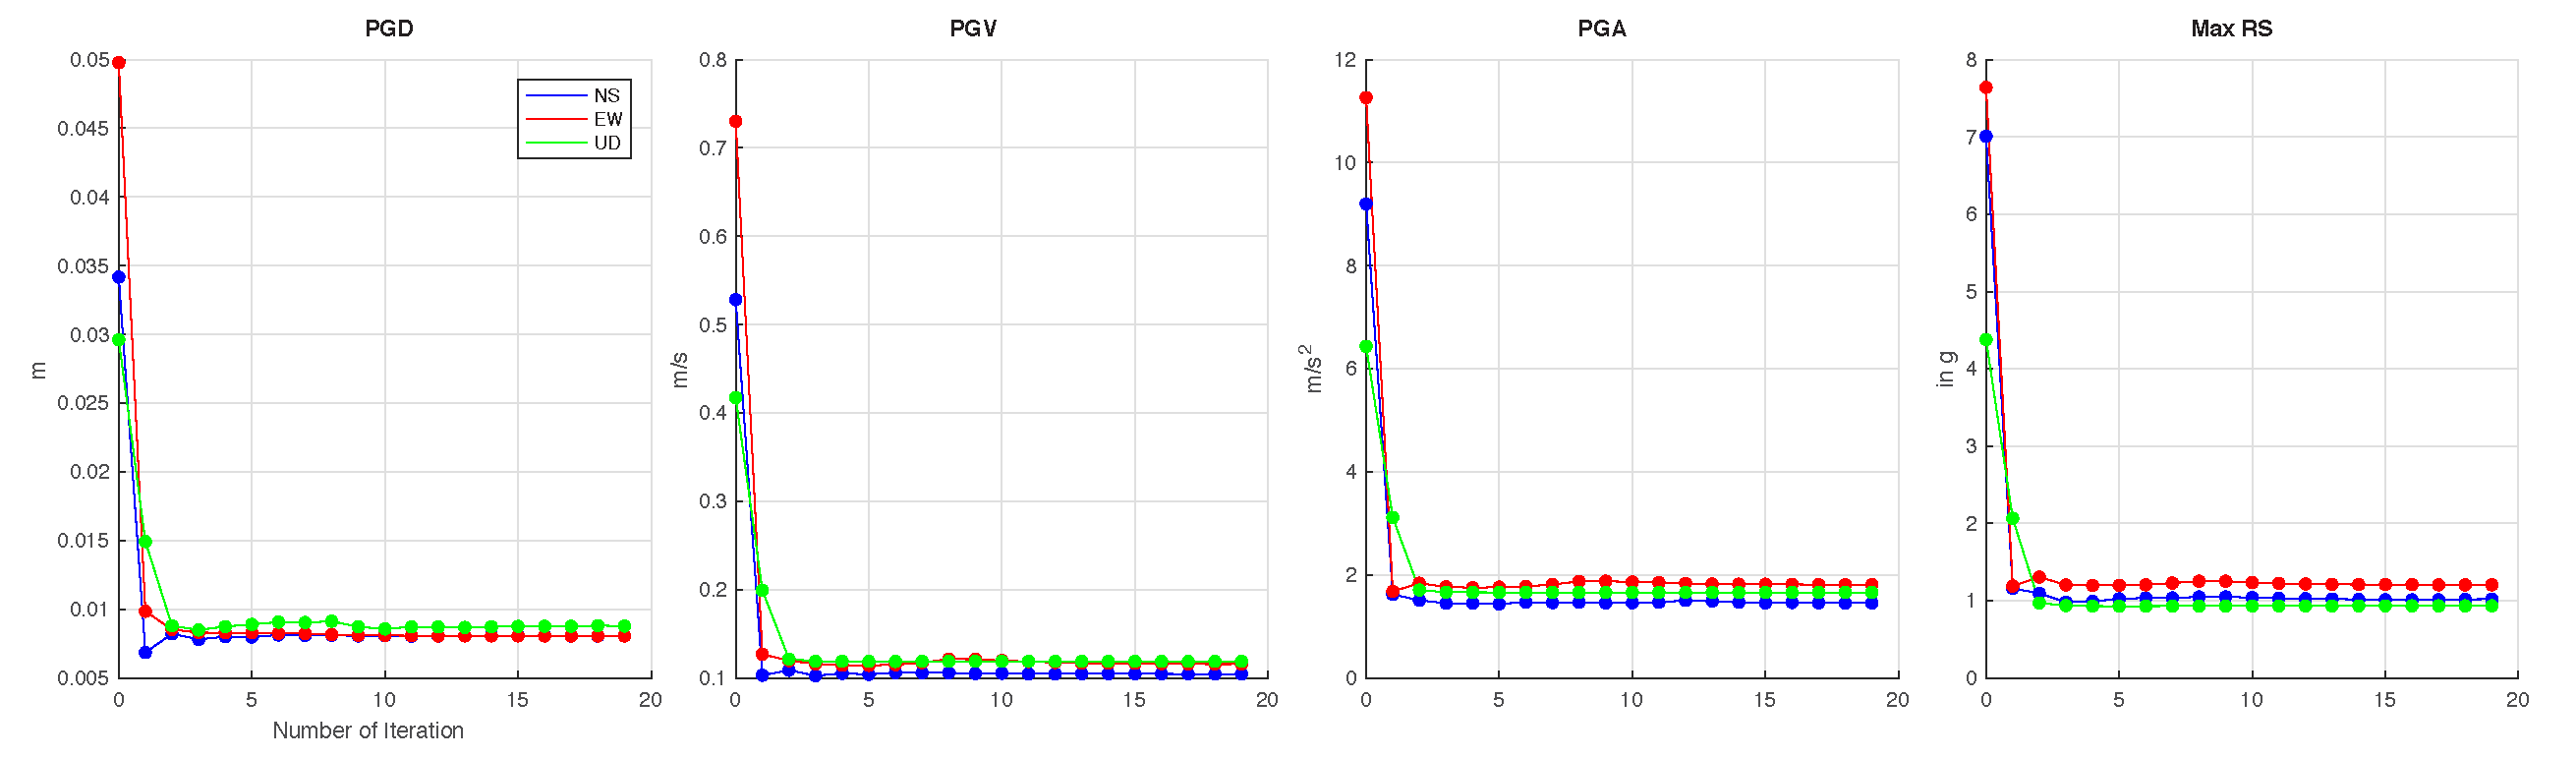
\includegraphics[width=\textwidth]{figures/pdf/iteration_deep_64.pdf}
    \caption{Analysis of stability of results in different iteration. Stations at the depth of 64 m.}
    \label{fig:iteration_deep_64}
\end{figure}


